% Op icon: polyline — chained straight segments through marked vertices.
\documentclass[tikz,border=2mm]{standalone}
\usetikzlibrary{arrows.meta,calc,shapes.geometric}
\begin{document}
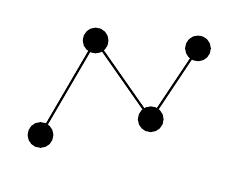
\begin{tikzpicture}[line width=1.3pt, line cap=round, line join=round, >=Stealth, x=1mm,y=1mm]
  \draw[thick] (-10,-6) -- (-3,6) -- (4,-4) -- (10,5);
  \foreach \p in {(-10,-6),(-3,6),(4,-4),(10,5)} { \filldraw \p circle (1.4); }
\end{tikzpicture}
\end{document}
